\chapter{Language: Context and Grounding}

\begin{learninggoals}
\item Explain why language tasks depend on deciding what linguistic structure must be preserved rather than on choosing an architecture by habit.
\item Use a context audit to decide whether token counts, local order, long-range context, or external grounding are needed.
\item Understand tokenization, bag-of-words, and n-grams as serious representation choices rather than as obsolete preprocessing steps.
\item Explain why contextual representations, sequence models, and transformers matter when meaning depends on surrounding language.
\item Distinguish generation quality from grounded, trustworthy behavior.
\item Distinguish a base language model from an instruction-following model and explain what additional training stages produce the behavioral difference.
\item Use a prompting strategy ladder to choose the simplest inference-time intervention that produces reliable behavior.
\item Choose among prompting, retrieval, and fine-tuning based on what kind of behavioral change is needed and what evidence is available.
\item Produce an NLP context-and-grounding card before making a serious NLP system claim.
\end{learninggoals}

The vision chapter treated invariance, shortcuts, and deployment realism as central problems. Language creates a parallel but different challenge. The same words can mean different things in different contexts, while the same idea can be expressed through very different surface forms. A language system therefore has to decide what may be collapsed away, what must be preserved, and when external grounding is required before fluent output can be trusted.

\begin{problemsolvinglens}
This chapter asks an NLP-specific modeling question: what linguistic structure must the task preserve, and what evidence shows that the system is using that structure rather than producing merely fluent behavior? The answer drives tokenization, baseline choice, contextual modeling, retrieval, and evaluation.
\end{problemsolvinglens}

By the end of the chapter, the reader should be able to write an NLP context-and-grounding card before claiming that a language system is ready.

\section{Opening Dilemma: Same Words, Different Meaning; Same Meaning, Different Words}

Suppose a university wants to build a course-support assistant for a large introductory course. Students send messages such as:
\begin{quote}
\texttt{I missed the lab because I was sick.}\\
\texttt{Can I still submit tonight?}
\end{quote}
\begin{quote}
\texttt{I was sick and missed today's lab.\\ Is late submission still possible?}
\end{quote}
The wording is different, but the underlying request is almost the same. Now compare those with:
\begin{quote}
\texttt{I missed the lab.}\\
\texttt{Does that affect my visa attendance record?}
\end{quote}
Surface overlap remains, but the operational meaning has changed sharply. One question may be answered from the course late-policy page. Another may require escalation to a human adviser because the institutional risk is different.

Language is difficult because surface form is not enough. The sentence \texttt{the bank approved the loan} uses the token \texttt{bank} differently from \texttt{the river reached the bank}. Meanwhile, two answers to the same question may use different wording while expressing the same underlying idea. If a model preserves too little structure, it collapses distinctions the task needs. If it preserves structure in the wrong way, it may sound fluent without being grounded, faithful, or useful.

This means NLP should not begin with model names. It should begin with a judgment question: what information must survive the representation? Some tasks care mainly about which words are present. Some care about local order such as negation. Some depend on long-range context, discourse, or entity reference. Some require external knowledge or retrieval before any answer can be trusted.

Throughout this chapter, keep one running case in view: a grounded course-support assistant. The same incoming student message may need to be categorized, matched to the correct policy passage, answered conservatively, or escalated to a human. That single workflow is useful because it shows why representation, retrieval, generation, grounding, and evaluation are not separate concerns in modern NLP.

\section{Problem-Solving Technique: Context Audit}

\begin{thinkingtool}
\textbf{Context audit.} Before choosing an NLP representation, write down:
\begin{itemize}[leftmargin=*]
\item whether token presence is enough,
\item whether local order matters,
\item whether long-range dependence matters,
\item whether external knowledge or retrieval is required,
\item whether dialect, register, or identity variation matters,
\item what output the task requires: a label, a span, a ranked list, or generated text.
\end{itemize}
\end{thinkingtool}

This is the chapter's most reusable habit. A bag-of-words baseline, an n-gram repair, a contextual encoder, or a retrieval-augmented generator are not interchangeable choices. They encode different claims about what linguistic structure matters. The context audit forces that claim onto the page before the model is built.

\begin{decisionbox}
In NLP, model choice should follow the context audit. If the task can safely collapse order and ambiguity, a sparse lexical baseline may be enough. If meaning depends on local or global context, the representation must preserve it. If correctness depends on outside facts, grounding becomes part of the system design rather than an optional upgrade.
\end{decisionbox}

\begin{practicalnote}
Workflow sketch: first decide whether token presence, local order, long-range context, or grounding matters. Then start with the simplest baseline that preserves the needed structure, add n-grams or contextual encoders if order and context matter, add retrieval if current evidence is required, and only then choose prompting, fine-tuning, or a hybrid after checking how the workflow will be evaluated.
\end{practicalnote}

\begin{thinkingtool}
\textbf{Artifact preview: NLP context-and-grounding card.} Keep six fields visible from the start: task type, output type, the linguistic structure that must survive, whether grounding is required, the escalation rule, and the evidence that would justify the final claim.
\end{thinkingtool}

\begin{thinkingtool}
\textbf{Wrong question $\rightarrow$ better question.} Wrong: ``Which NLP model is strongest?'' Better: ``What linguistic structure must survive, what evidence must be available at prediction time, and what kind of output does the workflow actually need?''
\end{thinkingtool}

\begin{thinkingtool}
\textbf{Signal to trust $\rightarrow$ signal to doubt.} Trust: the system retrieves the right evidence, preserves the task-relevant context, cites or exposes the source when needed, and escalates when the evidence is weak or the case is high risk. Doubt: the answer sounds fluent but the supporting passage is wrong, missing, stale, or never shown, and the workflow gives no safe way to abstain or defer.
\end{thinkingtool}

\begin{figure}[t]
\centering
\resizebox{0.95\linewidth}{!}{\definecolor{c9startBlue}{RGB}{56,103,170}
\definecolor{c9startBg}{RGB}{220,233,251}
\definecolor{c9decBg}{RGB}{237,231,250}
\definecolor{c9decLine}{RGB}{120,80,180}
\definecolor{c9methBg}{RGB}{210,238,220}
\definecolor{c9methLine}{RGB}{26,112,64}
\definecolor{c9ragBg}{RGB}{254,243,219}
\definecolor{c9ragLine}{RGB}{184,92,16}

\begin{tikzpicture}[x=1cm, y=1cm, font=\small,
  %% Start/end rectangles
  sbox/.style={draw=c9startBlue, fill=c9startBg, rounded corners=4pt,
               align=center, text width=2.7cm, minimum height=0.9cm,
               text=c9startBlue},
  %% Decision diamonds
  diam/.style={draw=c9decLine, fill=c9decBg, diamond, aspect=2.2,
               align=center, text width=2.5cm, minimum width=3.8cm, minimum height=1.0cm,
               font=\small, text=c9decLine, inner sep=2pt},
  %% Terminal method boxes
  mbox/.style={draw=c9methLine, fill=c9methBg, rounded corners=3pt,
               align=center, text width=2.5cm, minimum width=3.0cm, minimum height=0.9cm,
               text=c9methLine},
  %% RAG box (amber)
  rbox/.style={draw=c9ragLine, fill=c9ragBg, rounded corners=3pt,
               align=center, text width=2.7cm, minimum width=3.2cm, minimum height=0.9cm,
               text=c9ragLine},
  arr/.style={-Latex, thick, black!60},
  lbl/.style={font=\footnotesize, black!70, fill=white, inner sep=1pt},
]

%% ── Main spine (x=0) ─────────────────────────────────────────────────────
%%    2.8cm row spacing; diamonds centred; terminals branch left/right
\node[sbox] (start)     at (0,  0.0) {NLP task defined};
\node[diam] (tokens)    at (0, -2.8) {Is token presence enough?};
\node[diam] (order)     at (0, -5.6) {Does local order matter?};
\node[diam] (longrange) at (0, -8.4) {Need long-range context?};
\node[diam] (external)  at (0,-11.2) {Need external knowledge?};
\node[diam] (output)    at (0,-14.0) {What output shape?};

%% ── Left-branch terminals ────────────────────────────────────────────────
\node[mbox] (bow)       at (-5.0, -2.8) {Bag-of-words baseline};
\node[mbox] (ngram)     at (-5.0, -5.6) {n-gram sequence model};
\node[mbox] (contextual)at (-5.0, -8.4) {Contextual encoder};

%% ── Right-branch terminal ────────────────────────────────────────────────
\node[rbox] (rag)       at ( 5.0,-11.2) {Retrieval-augmented generation};

%% ── Bottom output terminals ──────────────────────────────────────────────
\node[mbox] (classify)  at (-3.2,-16.5) {Classification};
\node[mbox] (extract)   at ( 0.0,-16.5) {Span extraction};
\node[mbox] (generate)  at ( 3.2,-16.5) {Generation};

%% ── Main spine arrows ────────────────────────────────────────────────────
\draw[arr] (start)     -- (tokens);
\draw[arr] (tokens)    -- node[lbl,right] {No}  (order);
\draw[arr] (order)     -- node[lbl,right] {No}  (longrange);
\draw[arr] (longrange) -- node[lbl,right] {No}  (external);
\draw[arr] (external)  -- node[lbl,right] {No}  (output);

%% ── Yes branches (left) ──────────────────────────────────────────────────
\draw[arr] (tokens)    -- node[lbl,above] {Yes} (bow);
\draw[arr] (order)     -- node[lbl,above] {Yes} (ngram);
%% Purely horizontal Yes branch (contextual aligned with longrange)
\draw[arr] (longrange.west) -- node[lbl,above] {Yes} (contextual.east);

%% Contextual Encoder → External knowledge: clean L-bend down then right
\draw[arr] (contextual.south) -- ++(0,-0.8) -| (external.west);

%% ── Right Yes branch ─────────────────────────────────────────────────────
\draw[arr] (external.east) -- node[lbl,above] {Yes} (rag);

%% ── Output branches ──────────────────────────────────────────────────────
\draw[arr] (output.south west) -- node[lbl,left]  {Label}    (classify.north);
\draw[arr] (output.south)      -- node[lbl,right] {Span}     (extract.north);
\draw[arr] (output.south east) -- node[lbl,right] {Text}     (generate.north);

%% ── Complexity arrow: left of method boxes, label at arrow tip ────────────
\draw[-Latex, thick, black!50]
  (-6.9,-2.2) -- (-6.9,-13.8);
\node[font=\footnotesize\itshape, black!60, anchor=north, align=center]
  at (-6.9,-14.0) {increasing\\model complexity};

%% ── Context Audit annotation (far left, no overlap) ─────────────────────
\node[align=left, font=\footnotesize, black!65, text width=3.3cm]
  at (-9.6,-5.8) {%
  \textbf{Context Audit}\\[2pt]
  $\cdot$ token presence\\
  $\cdot$ local order\\
  $\cdot$ long-range context\\
  $\cdot$ external knowledge\\
  $\cdot$ dialect coverage\\
  $\cdot$ output format};

\end{tikzpicture}
}
\caption{Context audit flowchart for NLP representation choice. Each decision point corresponds to a key question in the context audit framework. The path through the flowchart determines the appropriate representation and model architecture, from simple bag-of-words baselines to retrieval-augmented generation systems.}
\label{fig:context-audit-flowchart}
\end{figure}

\section{Task Shape Before Representation Depth}

The first serious question in NLP is not ``which model is strongest?'' It is ``what behavior should the system produce?''

\subsection{Classification and Sequence Labeling}

Text classification assigns one label to a document or sentence: spam versus not spam, topic A versus topic B, positive versus negative. Sequence labeling assigns outputs to tokens or spans, such as named entities, part-of-speech tags, or extracted fields. Sequence labeling usually needs finer contextual precision because token meaning depends heavily on neighboring tokens.

\begin{example}[A Tiny Slot-Label Example]
Suppose the message is \texttt{I missed Lab 3 because I was sick tonight.}
A sequence labeler might assign labels like this:
\begin{center}
\begin{tabular}{@{}ll@{}}
\toprule
Token & Label \\
\midrule
\texttt{I} & O \\
\texttt{missed} & O \\
\texttt{Lab} & B-LAB \\
\texttt{3} & I-LAB \\
\texttt{because} & O \\
\texttt{I} & O \\
\texttt{was} & O \\
\texttt{sick} & B-REASON \\
\texttt{tonight} & B-TIME \\
\texttt{.} & O \\
\bottomrule
\end{tabular}
\end{center}
The exact tag set is not the point. The point is that the system must preserve token-level detail well enough to identify the lab reference, the reason, and the timing cue before it can route, retrieve, or answer safely.
\end{example}

\subsection{Retrieval and Ranking}

Some NLP systems are supposed to find relevant documents, passages, or answers rather than synthesize new text. In those cases, the output is a ranked list. This matters because evaluation should ask whether the right evidence was found, not only whether the final wording sounds plausible.

\begin{mathlens}
Suppose a retrieval system returns four passages with relevance labels \([0,1,0,1]\), and suppose there are three relevant passages in the whole collection.
\[
\mathrm{precision@2}=\frac{1}{2}, \qquad \mathrm{recall@4}=\frac{2}{3}, \qquad \mathrm{RR}=\frac{1}{2}.
\]
Precision@2 asks how clean the top of the list is, recall@4 asks how much of the relevant material the top four covered, and reciprocal rank cares only about where the first relevant passage appeared.
\end{mathlens}

\subsection{Translation, Summarization, Question Answering, and Generation}

Machine translation must preserve meaning while changing surface form. Summarization must compress content without inventing unsupported claims. Question answering may require retrieval, reasoning, or synthesis across several passages. Open-ended generation asks the system to continue, rewrite, or compose text under a prompt. These tasks differ sharply in what counts as success.

Question answering itself can be extractive, templated, or generative. An extractive system copies a span from the source, a templated system fills a bounded slot, and a generative system composes a freer response. The safest output style depends on how much wording freedom the task actually allows.

\begin{example}[Why Task Shape Comes First]
A course-support assistant may be built in at least three different ways. It might classify messages into categories such as \emph{deadline}, \emph{grading}, or \emph{technical issue}; retrieve the most relevant syllabus or policy passage; or generate a direct response for the student. Those are not cosmetic differences. They define different outputs, different evaluation standards, and different failure modes.
\end{example}

\begin{decisionbox}
\textbf{Choose the smallest NLP workflow that preserves the needed structure.}
\begin{itemize}[leftmargin=*]
\item Stable lexical cues and label output: start with bag-of-words or n-grams.
\item Token-level extraction or strong local-order dependence: sequence labeling or contextual encoders.
\item Long-range context, paraphrase, or discourse dependence: contextual sequence models or transformers.
\item Correctness depends on current documents or policies: retrieval must be part of the system.
\item Output is a controlled transformation of source text: encoder-decoder modeling is a natural fit.
\end{itemize}
\end{decisionbox}

\section{Worked Workflow: One Message, Several NLP Jobs}

The running case becomes clearer when the whole workflow is written down. Consider the message
\begin{quote}
\texttt{I missed Lab 3 because I was sick.\\ Can I submit tonight without penalty?}
\end{quote}
The system should not jump directly from raw text to a fluent answer. It usually has to solve several smaller NLP problems in sequence. Figure~\ref{fig:course-support-pipeline} gives the high-level pipeline, while Table~\ref{tab:course-support-workflow} names the main subproblems more explicitly.

\begin{figure}[t]
\centering
\resizebox{\linewidth}{!}{%
\begin{tikzpicture}[
  font=\small,
  box/.style={draw, rounded corners, align=center, minimum height=0.9cm, minimum width=2.0cm, fill=black!4},
  arrow/.style={-Latex, thick}
]
\node[box] (message) {Student\\message};
\node[box, right=0.8cm of message] (routing) {Intent\\routing};
\node[box, right=0.8cm of routing] (slots) {Key\\details};
\node[box, right=0.8cm of slots] (retrieval) {Retrieve\\policy};
\node[box, below=1.2cm of retrieval] (decision) {Answer or\\escalate};
\node[box, below left=0.95cm and 0.45cm of decision] (answer) {Grounded\\response};
\node[box, below right=0.95cm and 0.45cm of decision] (human) {Human\\specialist};
\node[box, left=1.1cm of decision] (source) {Syllabus and\\policy index};

\draw[arrow] (message) -- (routing);
\draw[arrow] (routing) -- (slots);
\draw[arrow] (slots) -- (retrieval);
\draw[arrow] (retrieval) -- (decision);
\draw[arrow] (source) -- (decision);
\draw[arrow] (decision) -- (answer);
\draw[arrow] (decision) -- (human);
\end{tikzpicture}%
}
\caption{A grounded language workflow does not move directly from message to fluent reply. It routes the request, preserves task-relevant details, retrieves authoritative evidence, and only then decides between bounded automation and escalation.}
\label{fig:course-support-pipeline}
\end{figure}

\begin{table}[t]
\centering
\small
\setlength{\tabcolsep}{3pt}
\renewcommand{\arraystretch}{1.08}
\begin{tabular}{@{}>{\raggedright\arraybackslash}p{2.11cm}>{\raggedright\arraybackslash}p{2.36cm}>{\raggedright\arraybackslash}p{5.9cm}@{}}
\toprule
Stage & Typical output & Role in the workflow \\
\midrule
Intent routing & \texttt{deadline}, \texttt{extension} & Separates routine policy requests from disputes, technical issues, visa questions, or wellbeing cases \\
Entity or slot reading & \texttt{Lab 3}, \texttt{illness}, \texttt{tonight} & Preserves the details that control retrieval, escalation, and answer wording \\
Retrieval & syllabus or illness-policy passages & Adds current institutional evidence before any answer is written \\
Policy decision & answer directly or escalate & Marks which cases are safe to automate and which must go to a human specialist \\
Grounded response generation & brief answer tied to evidence & Produces readable language that stays faithful to the retrieved text \\
\bottomrule
\end{tabular}
\caption{One support message often activates several NLP subproblems, not just one. This is why Chapter 8 needs classification, retrieval, generation, grounding, and escalation in the same conceptual frame.}
\label{tab:course-support-workflow}
\end{table}

Now compare the same workflow for the message
\begin{quote}
\texttt{I missed the lab. Does that affect my visa attendance record?}
\end{quote}
The lexical overlap is high, but the correct system behavior may be completely different. A direct answer may be unsafe because the question is both higher stakes and more dependent on individual institutional context. The right system may still classify the message, retrieve the most relevant advising page, and then route the student to a human specialist rather than generating a confident answer on its own.

\begin{practicalnote}
In modern NLP systems, the model is often only one stage in a language workflow. The chapter is easier to read if students keep asking: what subproblem is being solved at this stage, and what later stage depends on it?
\end{practicalnote}

\section{Tokenization as a Modeling Decision}

Machine-learning models do not receive meaning directly. They receive tokenized input. Tokenization converts raw text into units such as words, subwords, or characters, and that choice changes what the model is allowed to notice and reuse.

\begin{center}
\emph{Tokenization decides what the model is allowed to notice and reuse.}
\end{center}

\subsection{Why Tokenization Matters}

Consider the strings \texttt{unbelievable}, \texttt{un-believable}, and \texttt{un believable}. A word-level tokenizer may treat them as distinct whole tokens. A subword tokenizer may expose shared pieces such as \texttt{un} and \texttt{believe}. A character-level model may see only letters. Each choice changes what the model can generalize across and what it must memorize.

The same issue appears in support messages. Strings such as \texttt{late-day}, \texttt{late day}, \texttt{lab-3}, and \texttt{CS101} contain structure that may be split, preserved, or blurred depending on the tokenizer. If the tokenizer handles course codes, dates, or policy terms poorly, the system may fail before the main language model has had any chance to reason well.

\begin{prereqbridge}
For this chapter, it is enough to think of a token as a unit the model can read. A document becomes a sequence $(w_1, w_2, \ldots, w_T)$ of such units, and the sequence length $T$ can vary from one example to another.
\end{prereqbridge}

Tokenization is therefore not clerical preprocessing. It is part of the representation claim. A bad tokenization choice can erase useful regularity before the main model has even started learning.

\section{Bag-of-Words as the First Serious Lexical Baseline}

\begin{definition}[Bag-of-Words Representation]
A bag-of-words representation maps text to token counts while discarding token order.
\end{definition}

Suppose the vocabulary contains $V$ tokens. A document is mapped to a vector $x \in \mathbb{R}^{V}$ whose component $x_j$ records how often vocabulary item $j$ appears. This sounds simple because it is simple. That is exactly why it remains a valuable baseline. If the task depends mainly on broad lexical content, topic markers, or keyword presence, bag-of-words can work well.

\begin{mathlens}
Take the two sentences \texttt{dog bites man} and \texttt{man bites dog}. If the unigram vocabulary is ordered as \texttt{[dog, bites, man]}, then both sentences have the same count vector
\[
x_{\text{uni}}=(1,1,1).
\]
Now use a bigram vocabulary with four entries:
\texttt{dog bites}, \texttt{bites man}, \texttt{man bites}, and \texttt{bites dog}. The first sentence has
\[
x_{\text{bi}}=(1,1,0,0),
\]
while the second has
\[
x_{\text{bi}}=(0,0,1,1).
\]
Bag-of-words collapses the order distinction; bigrams repair exactly that local structure.
\end{mathlens}

For the running support-assistant case, bag-of-words can already be a serious routing baseline. Messages containing words such as \texttt{grade}, \texttt{rubric}, \texttt{deadline}, \texttt{extension}, \texttt{compile}, or \texttt{autograder} often reveal a lot about which queue or policy family is relevant. That does not make bag-of-words sufficient for the whole system, but it does make it a meaningful first rung on the baseline ladder.

\subsection{Worked Example: Same Words, Different Meaning}

Consider the two sentences
\begin{quote}
\texttt{dog bites man}\\
\texttt{man bites dog}
\end{quote}
Their bag-of-words vectors are identical. Both contain one occurrence of \texttt{dog}, one of \texttt{bites}, and one of \texttt{man}. Yet their meanings are very different.

This example matters because it teaches the right judgment rule. A representation is not evaluated by whether it sounds sophisticated. It is evaluated by whether it preserves the distinctions the task requires. If the task is broad topic detection, bag-of-words may be enough. If the task is to identify who acted on whom, it is inadequate.

\begin{example}[Bag-of-Words Can Still Be Strong for Routing]
Suppose the course-support system must first route messages into \emph{deadline}, \emph{grading}, \emph{technical issue}, or \emph{administrative request}. A message containing \texttt{deadline}, \texttt{extension}, and \texttt{submission} may be routable quite well with bag-of-words alone. That is a real success, not an embarrassment. It shows that some tasks depend mainly on lexical content even if later grounded answering requires more structure.
\end{example}

\begin{figure}[t]
\centering
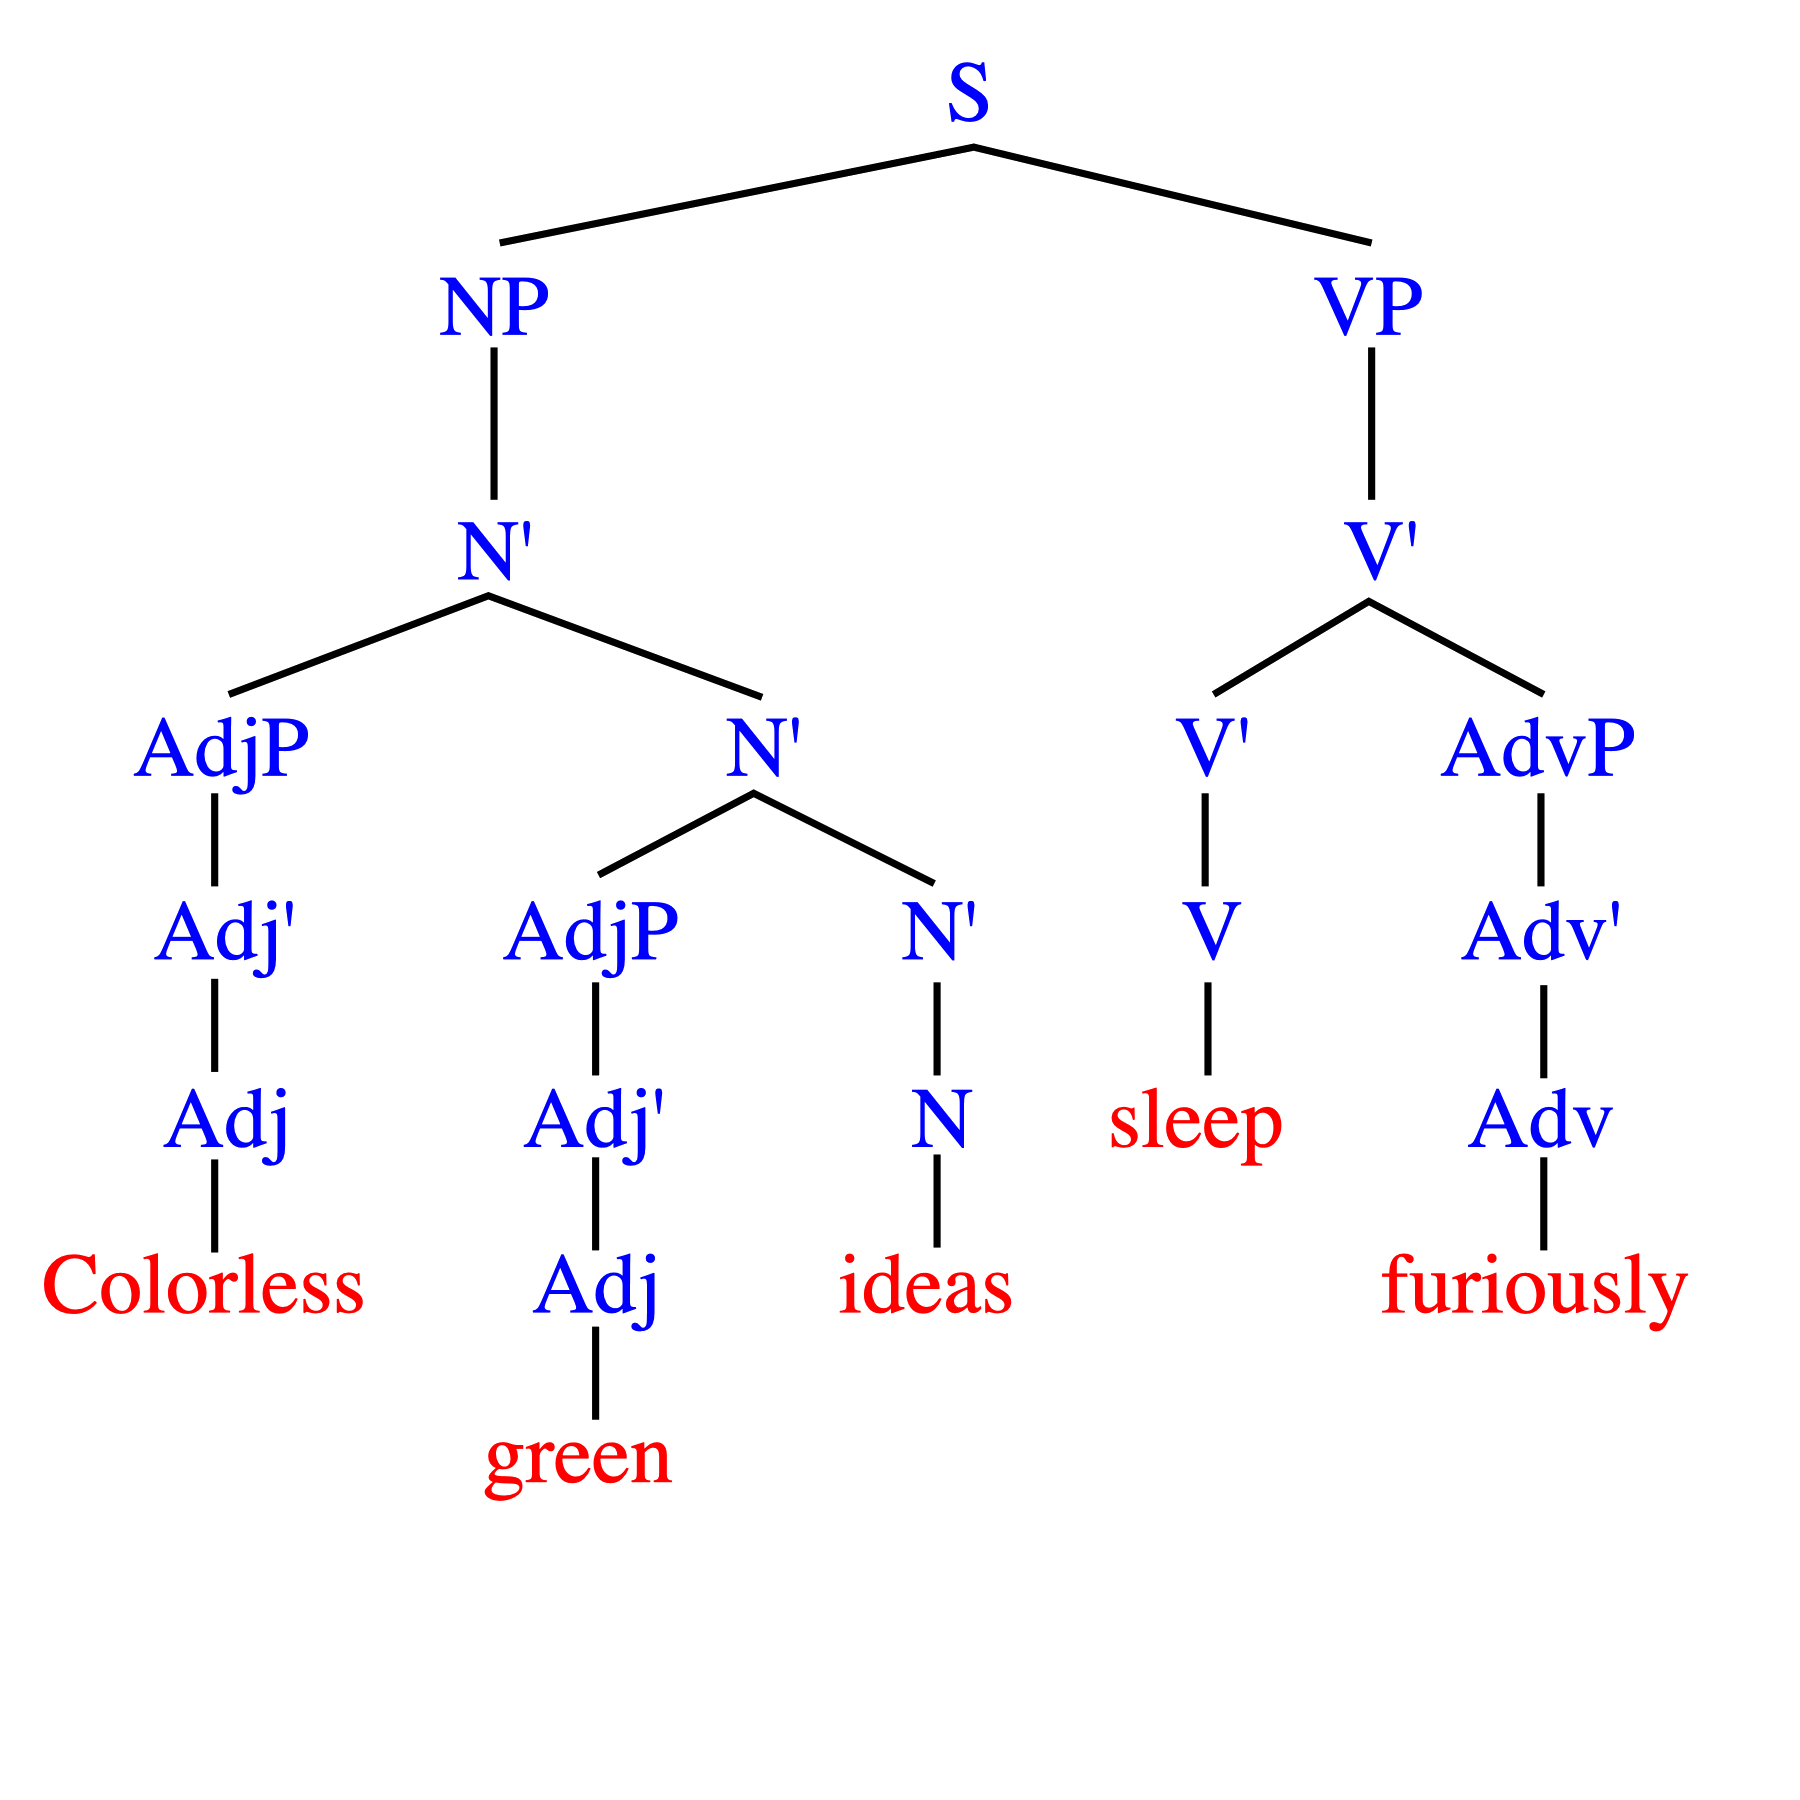
\includegraphics[width=0.66\linewidth]{figures/external/syntax_tree_clean.png}
\caption{A syntax tree is one visual reminder that sentences contain internal structure beyond token counts. The example sentence is ``Colorless green ideas sleep furiously.'' Public-domain image from Wikimedia Commons \citep{wikimedia_syntax_tree}.}
\label{fig:syntax-tree-visual}
\end{figure}

The point is not that every useful NLP system must build an explicit parse tree. The point is that language has compositional structure, and a bag-of-words vector cannot record which words group together or which phrases modify which others.

\begin{failurebox}
Bag-of-words is not ``dead.'' It is a strong baseline when token presence carries most of the signal. It fails when the task depends on distinctions that token counts erase.
\end{failurebox}

\section{N-Grams as the Local-Order Repair}

One classical way to restore some order information is to use n-grams. A unigram is a single token, a bigram is an adjacent token pair, and a trigram is a length-three token sequence. Including bigrams lets the model distinguish between \texttt{dog bites} and \texttt{bites dog}, which plain bag-of-words cannot.

\begin{center}
\emph{If the needed context is local, repair the representation before escalating the model family.}
\end{center}

This is one of the chapter's main modeling lessons. Some problems that appear to require deep architectures can be solved by preserving a little more local structure. N-grams are therefore not just historical trivia. They are evidence that the missing structure may be local rather than global.

\begin{example}[Local Order Matters in Policy Language]
Consider the phrases \texttt{late submission allowed} and \texttt{late submission not allowed}. A unigram representation treats both as nearly the same bag of words and can understate the force of the local negation. A bigram feature such as \texttt{not allowed} repairs exactly that kind of short-range structural loss. This is why n-grams remain conceptually important: sometimes the missing structure is not broad world knowledge but one small local dependency with operational consequences.
\end{example}

\section{From Static to Contextual Meaning}

Bag-of-words and n-grams produce sparse count vectors. Modern NLP often uses dense embeddings instead.

\begin{definition}[Word Embedding]
A word embedding is a dense vector representation of a token learned so that tokens occurring in similar contexts receive similar vectors.
\end{definition}

In modern NLP, \emph{word} is often shorthand for \emph{token}: the embedding may correspond to a word, a subword piece, or even a character, depending on the tokenizer.

Embeddings allow statistical sharing across related words. If \texttt{exam}, \texttt{quiz}, and \texttt{test} occur in similar contexts, their vectors may become nearby in embedding space. This makes downstream learning easier when exact lexical overlap is limited.

\subsection{Static Embeddings}

Static embeddings assign one vector per word type. This is already much more expressive than isolated one-hot vectors, but it still has a serious limitation: a token receives the same representation regardless of where it appears.

\subsection{Contextual Representations}

Contextual models allow a token's representation to depend on the surrounding text. This is one of the deepest shifts in modern NLP.

\begin{example}[Why Contextualization Matters]
In the sentence \texttt{the bank approved the loan}, surrounding words suggest a financial institution. In \texttt{the river reached the bank}, surrounding words suggest a geographic boundary. A contextual model can represent these two uses differently even though the surface token \texttt{bank} is the same.
\end{example}

The same issue appears in the running case. The token \texttt{extension} may refer to a deadline extension, a visa extension, or an extension number for a campus office. A good support assistant should not collapse those meanings merely because the same surface word appears. The surrounding language determines which workflow, evidence source, and risk level are appropriate.

\begin{center}
\emph{A contextual representation does not assign meaning to a word in isolation; it computes meaning inside a sentence.}
\end{center}

\section{Sequence Models and Attention as Context Builders}

Once text is treated as a sequence rather than a bag, the next question is how context is carried.

\subsection{Recurrent Models}

Recurrent neural networks and LSTMs process text one token at a time while carrying forward a hidden state. Conceptually, that hidden state summarizes what has been seen so far. These models were historically important because they made context explicit, but they also showed the limitation of compressing long sequences into a moving state.

\subsection{Attention and Transformers in NLP}

Transformers became dominant in NLP because attention allows each token representation to look directly at other tokens that matter, rather than relying only on a compressed recurrent summary. If a pronoun depends on a noun many words earlier, or a negation changes the sentiment of a later phrase, attention provides a flexible way to connect those pieces.

This is why transformer-based pretraining changed the field so quickly \citep{vaswani2017,devlin2019}. The important idea is not that attention is magical. It is that contextual representation learning became far more scalable and reusable.

\begin{advancednote}
Chapter 6 already explained attention as a general representation mechanism. In NLP, the central point is task-specific: attention matters because token meaning often depends on distant and selective context, not merely on adjacent words.
\end{advancednote}

\section{Language Modeling as Sequence Prediction}

\begin{definition}[Language Model]
A language model assigns probabilities to sequences of tokens, typically by predicting each next token conditioned on the tokens that came before it.
\end{definition}

This chapter uses the classic autoregressive setup because it makes the next-token logic explicit. Masked or denoising objectives are also important in modern NLP, but the next-token factorization is the clearest starting point for the sequence-prediction story here.

If a sequence is $(w_1, w_2, \ldots, w_T)$, a standard factorization is
\[
P(w_1, w_2, \ldots, w_T) = \prod_{t=1}^{T} P(w_t \mid w_1, \ldots, w_{t-1}).
\]
Conceptually, language modeling asks one repeated question: given the text so far, what token should come next?

\begin{mathlens}
If the model assigns probabilities \(p_t=P(w_t\mid w_1,\ldots,w_{t-1})\) to the observed tokens, then the sequence probability is \(\prod_{t=1}^T p_t\). The average negative log-likelihood is
\[
\mathrm{NLL}=-\frac{1}{T}\sum_{t=1}^T \log p_t,
\]
and perplexity is
\[
\mathrm{PP}=\exp(\mathrm{NLL})=\left(\prod_{t=1}^T p_t\right)^{-1/T}.
\]
So perplexity is the inverse geometric mean probability per token: lower is better because the model assigned higher probability to the observed sequence.
\end{mathlens}

Perplexity comparisons are only meaningful when tokenization and evaluation protocol are held fixed. A model scored on subword units is not directly comparable to a model scored on different tokens unless the setup is normalized carefully.

\subsection{Worked Example: A Tiny Bigram Model}

Suppose a tiny corpus contains the following counts after the token \texttt{bank}:
\[
\texttt{approved}: 6, \qquad \texttt{loan}: 1, \qquad \texttt{closed}: 3.
\]
A simple bigram model estimates
\[
P(\texttt{approved} \mid \texttt{bank}) = \frac{6}{10} = 0.6.
\]
If the current context ends with \texttt{bank}, then \texttt{approved} is the most likely next token under this tiny model.

The example is deliberately simple, but it teaches the core logic cleanly. Generation is repeated sequence prediction, not mysterious text magic.

\subsection{Encoder-Decoder Models as Conditional Sequence Mapping}

Not every language task is best understood as open-ended continuation. Translation and summarization are better viewed as conditional sequence mapping: the input sequence is the evidence or source text, and the output sequence is a new sequence whose content must be constrained by that source.

In that setting, the model is not primarily asking, ``What token comes next in this text?'' It is asking, ``Given this source sequence, what target sequence should be produced?'' That difference matters because the output is judged against the input's meaning, not only against local continuation plausibility.

\begin{center}
\emph{Next-token prediction extends text. Conditional sequence mapping transforms one sequence into another.}
\end{center}

The architecture can be kept conceptually light: an encoder reads the source, a decoder writes the target, and the source remains available as the main conditioning signal throughout generation. The important modeling decision is not the machinery itself. It is whether the task shape is source-to-target transformation or free continuation.

\begin{mathlens}
For a source sequence \(x\) and target sequence \(y=(y_1,\ldots,y_T)\), the conditional generation objective is
\[
P(y\mid x)=\prod_{t=1}^{T} P(y_t \mid y_1,\ldots,y_{t-1},x).
\]
Training therefore rewards target tokens that are correct given both the source and the already-generated prefix. The source is not background context. It is part of the probability model.
\end{mathlens}

\begin{codeexample}[caption={A minimal encoder-decoder training sketch}]
encode the source sequence x
for each target position t:
    use the source representation and previous target tokens
    predict the next target token y_t
    add loss for the correct y_t
update encoder and decoder parameters
\end{codeexample}

\begin{example}[Tiny Translation Example]
Input: \texttt{The student missed the lab because of illness.}\\
Output: \texttt{Der Student verpasste das Labor wegen Krankheit.}

The output is not a continuation of the English sentence. It is a constrained transformation into another language. The source sentence provides the evidence that must be preserved, while the target sentence must be fluent in the new language.
\end{example}

\begin{example}[Tiny Summarization Contrast]
Source: \texttt{Late work due to illness is possible only after the extension form is filed within forty-eight hours.}\\
Good summary: \texttt{Illness extensions require a form within forty-eight hours.}\\
Bad summary: \texttt{Illness always allows late work.}

The bad summary sounds plausible, but it drops the operational constraint that the source required. This is exactly the kind of failure that sequence transformation can hide if the model is fluent but not faithful.
\end{example}

\begin{practicalnote}
Choose encoder-decoder structure when the task has a clear source text and a target text with different surface form but preserved content, such as translation, abstractive summarization, or controlled rewriting. Plain continuation is a better fit when the system should extend an already-open prompt, improvise within the prompt's style, or generate text without a fixed source-output boundary.
\end{practicalnote}

\begin{practicalnote}
The evidence question also changes. In continuation, the prompt itself is usually the main context. In sequence transformation, the source text is evidence that constrains the whole output, and any retrieval you add should support that source rather than replace it.
\end{practicalnote}

\begin{warningbox}
Encoder-decoder structure does not guarantee faithfulness. If the target is freer than the source permits, the model can compress away conditions, hedge too little, or invent support that was never in the source. High-risk tasks may therefore require extraction, citation, or grounded answer policies even when encoder-decoder modeling fits the task shape well.
\end{warningbox}

\section{Decoding, Retrieval, and Grounding as Behavior Design}

Once a language model produces next-token probabilities, the system still needs a behavior policy.

\subsection{Decoding Changes the Behavior}

Greedy decoding always picks the highest-probability next token. Sampling introduces randomness. Temperature changes how conservative or diverse the output becomes. Two systems built on the same model can therefore behave very differently depending on decoding choices.

\subsection{Retrieval and Grounding Change the Claim}

Fluent continuation is not enough when correctness depends on trustworthy outside information. In those settings, retrieval and grounding are not optional embellishments. They change what the system is allowed to claim.

This is the deeper reason retrieval-augmented generation matters. Once a language system is required to retrieve evidence before answering, the strongest defensible claim is no longer ``the model knows the answer.'' It is narrower and more technical: given the current document collection, retrieval pipeline, and answer policy, the system can often find the right supporting material and stay faithful to it \citep{lewis2020rag}. That claim is better because it can be audited. It also means many apparent language failures are really retrieval or policy failures earlier in the pipeline.

\begin{figure}[t]
\centering
\definecolor{c9l1Line}{RGB}{120,130,145}
\definecolor{c9l1Bg}{RGB}{242,244,246}
\definecolor{c9l2Line}{RGB}{56,103,170}
\definecolor{c9l2Bg}{RGB}{220,233,251}
\definecolor{c9l3Line}{RGB}{26,112,64}
\definecolor{c9l3Bg}{RGB}{210,238,220}
\definecolor{c9l4Line}{RGB}{184,92,16}
\definecolor{c9l4Bg}{RGB}{254,237,215}
\resizebox{\linewidth}{!}{%
\begin{tikzpicture}[x=1cm, y=1cm, font=\small,
  r1/.style={draw=c9l1Line, fill=c9l1Bg, rounded corners=4pt,
             align=left, text width=8.0cm, minimum height=1.0cm, inner sep=7pt},
  r2/.style={draw=c9l2Line, fill=c9l2Bg, rounded corners=4pt,
             align=left, text width=8.0cm, minimum height=1.0cm, inner sep=7pt},
  r3/.style={draw=c9l3Line, fill=c9l3Bg, rounded corners=4pt,
             align=left, text width=8.0cm, minimum height=1.0cm, inner sep=7pt},
  r4/.style={draw=c9l4Line, fill=c9l4Bg, rounded corners=4pt,
             align=left, text width=8.0cm, minimum height=1.0cm, inner sep=7pt},
  arr/.style={-Latex, thick, black!45}
]
\node[r1] (bow)     at (0, 0.0) {%
  \textcolor{c9l1Line}{\textbf{1}}\enspace
  \textbf{Bag-of-words:} preserves token presence; often enough for first-pass routing};
\node[r2, above=0.4cm of bow] (ngram) {%
  \textcolor{c9l2Line}{\textbf{2}}\enspace
  \textbf{N-grams:} restore local order when short dependencies such as \texttt{not allowed} matter};
\node[r3, above=0.4cm of ngram] (context) {%
  \textcolor{c9l3Line}{\textbf{3}}\enspace
  \textbf{Contextual representations:} disambiguate sentence meaning when a token such as \texttt{extension} changes role with context};
\node[r4, above=0.4cm of context] (ground) {%
  \textcolor{c9l4Line}{\textbf{4}}\enspace
  \textbf{Retrieval and grounding:} attach the answer to current external evidence when the model should not rely on internal plausibility alone};
%% Upward arrows between rungs
\draw[arr] (bow)     -- (ngram);
\draw[arr] (ngram)   -- (context);
\draw[arr] (context) -- (ground);
\end{tikzpicture}%
}
\caption{The chapter's representation ladder moves from token presence to local order, sentence context, and finally grounded external evidence. The right choice is not always the top rung; it is the smallest rung that preserves the structure the task truly needs.}
\label{fig:nlp-representation-ladder}
\end{figure}

\begin{center}
\emph{In NLP, behavior is determined not only by the model, but also by decoding policy and by whether the system is grounded.}
\end{center}

\begin{example}[Grounded Versus Ungrounded Answering]
Suppose a student asks a course-support assistant, ``I missed Lab 3 because I was sick. Can I submit tonight without penalty?'' A pure generator may produce a fluent answer from internal statistical patterns alone, such as ``Yes, illness usually allows a late submission.'' A grounded system instead retrieves the current course late-policy page and conditions the answer on that source. The second system supports a stronger claim because its output can be traced to current evidence rather than to generic linguistic plausibility.
\end{example}

\subsection{Retrieval Contract: What Evidence Must Be Present?}

In grounded systems, retrieval quality is not only about whether something relevant appears somewhere in the top few results. The stronger question is whether the retrieved evidence is good enough to support the answer policy the system is about to use.

\begin{thinkingtool}
\textbf{Retrieval contract.} Before trusting a grounded answer, ask four questions: was the right passage retrieved, was it authoritative, was it current, and was it complete enough to support the answer without hidden conditions or missing exceptions?
\end{thinkingtool}

This matters because retrieval failure is not only absence. The system can retrieve a plausible-looking but stale page, a related but incomplete rule, or a fragment that omits the condition that changes the whole answer. A top-ranked result may therefore look linguistically relevant while still violating the operational contract of the task.

\begin{table}[t]
\centering
\small
\setlength{\tabcolsep}{4pt}
\begin{tabular}{p{2.32cm}p{3.32cm}p{4.31cm}}
\toprule
Contract element & What must be true & Typical failure if it is missing \\
\midrule
Relevance & The passage addresses the user's actual policy or factual question & The answer is fluent but about the wrong rule \\
Authority & The source is one the organization is willing to stand behind & The system cites unofficial or low-trust material \\
Freshness & The passage is current for the semester, product version, or policy window that matters & The answer is correct for last term and wrong for this one \\
Completeness & The evidence includes the conditions, exceptions, and escalation path needed for action & The answer omits the one clause that changes what the user should do \\
\bottomrule
\end{tabular}
\caption{A grounded answer is only as good as the retrieval contract behind it. Hit rate alone does not tell the whole story.}
\label{tab:retrieval-contract}
\end{table}

\subsection{Retrieval Pipeline Anatomy}

A practical retrieval stack usually has five stages:
\begin{itemize}[leftmargin=*]
\item \textbf{Chunking.} Split documents into passages that can be searched; too coarse hides the right sentence, too fine removes surrounding conditions.
\item \textbf{Indexing.} Build a lexical or vector index so the system can search quickly.
\item \textbf{First-pass retrieval.} Pull a broad candidate set using a cheap similarity score.
\item \textbf{Reranking.} Rescore the candidates with a stronger model or additional features.
\item \textbf{Grounding and citation.} Answer only from the selected evidence, and expose the source when the user or reviewer needs an audit trail.
\end{itemize}

\begin{practicalnote}
If chunking strips away the exception clause, no reranker can recover it later. Retrieval quality starts with how the evidence was segmented.
\end{practicalnote}

Once this contract is stated explicitly, retrieval evaluation becomes sharper. A system should not get full credit merely because a vaguely related document appeared somewhere in the ranking. The document must be the right kind of support for the answer the system is going to present.

\subsection{Retrieval Failure Often Precedes Generation Failure}

In grounded language systems, a bad final answer is often a retrieval failure in disguise. The answer may read smoothly while being based on the wrong policy passage, an outdated FAQ, or no real support at all. This matters because otherwise teams over-diagnose the generator and under-diagnose the evidence path.

\begin{table}[t]
\centering
\small
\setlength{\tabcolsep}{4pt}
\begin{tabular}{p{2.51cm}p{3.18cm}p{4.26cm}}
\toprule
Pipeline failure & What the answer may look like & What actually failed \\
\midrule
No relevant passage retrieved & Fluent but unsupported answer & The generator had no authoritative evidence to ground on \\
Wrong passage ranked first & Confident answer to the wrong rule & Lexical overlap looked plausible, but the operational intent was missed \\
Current and stale passages mixed & Contradictory or hedged answer & The evidence set itself was inconsistent \\
High-risk case not escalated & Polite but unsafe direct answer & The behavior policy failed, not only the language model \\
\bottomrule
\end{tabular}
\caption{In grounded NLP, many answer failures begin as retrieval or escalation failures before they become generation failures.}
\label{tab:nlp-retrieval-failure-modes}
\end{table}

\begin{example}[Same Generator, Different Evidence]
Suppose the same language model is used twice on the question ``Can I submit tonight without penalty?'' In one run, retrieval returns the current late-policy page and the illness-extension instructions. In another, retrieval returns an outdated FAQ plus a general attendance page. The generator may be identical in both cases, yet the second run is much more likely to produce a polished but operationally wrong answer. That is why grounded systems must be evaluated as pipelines rather than as text generators alone.
\end{example}

\subsection{Escalation and Abstention Change the Behavior Too}

Sometimes the right language-system behavior is not to answer directly at all. A message about visa attendance, harassment, self-harm, disability accommodation, or grade appeal may require specialized context, a stronger audit trail, or institutional authority that the model does not have. In those cases, the right system may classify the request, retrieve supporting information for the human reviewer, and abstain from final answering.

\begin{practicalnote}
Generation is only one possible output policy. In support systems, a good abstention or escalation rule can be more valuable than a slightly more fluent answerer.
\end{practicalnote}

\begin{practicalnote}
When evidence is weak, good grounded systems usually tighten behavior rather than loosen it. They answer with explicit support, answer conservatively, or abstain. They should not answer boldly from uncertain retrieval.
\end{practicalnote}

\begin{failurebox}
Fluency is not proof of truth. A system can produce coherent, confident language while relying on weak context, unsupported continuation patterns, or stale internal knowledge.
\end{failurebox}

\section{From Language Model to Instruction-Following Model}

A language model trained only on next-token prediction learns to continue text in ways that are statistically plausible given its training distribution. That is a useful foundation, but it is not yet a system that follows instructions, answers questions reliably, or behaves consistently across diverse inputs. The gap between a base language model and an instruction-following system requires additional training stages that apply different kinds of behavioral pressure.

\begin{center}
\emph{A base language model predicts likely continuations. An instruction-following model responds to requests in a way that is helpful, bounded, and consistent.}
\end{center}

This distinction matters because the two systems have different failure modes. A base model produces text that is statistically plausible but may be factually wrong, harmful in some contexts, or unresponsive to the intent behind an input. An instruction-following model is shaped to interpret and respond to the intent behind a request, but it may still hallucinate, behave inconsistently under paraphrase, or fail when inputs differ structurally from those seen during alignment.

\begin{figure}[t]
\centering
\resizebox{\linewidth}{!}{%
\begin{tikzpicture}[
  font=\small,
  stage/.style={draw, rounded corners, align=center, minimum height=1.1cm, minimum width=3.0cm, fill=black!4},
  sublabel/.style={align=center, text width=3.0cm, font=\footnotesize},
  superlabel/.style={align=center, text width=3.0cm, font=\footnotesize},
  arrow/.style={-Latex, thick}
]
\node[stage] (pre)   at (0.0, 0) {Pretraining\\on broad text};
\node[stage] (sft)   at (4.6, 0) {Instruction\\fine-tuning};
\node[stage] (align) at (9.2, 0) {Preference\\alignment};

\draw[arrow] (pre)   -- (sft);
\draw[arrow] (sft)   -- (align);

\node[superlabel] at (0.0,  1.6) {unlabeled text at\\large scale};
\node[superlabel] at (4.6,  1.6) {curated (instruction,\\response) pairs};
\node[superlabel] at (9.2,  1.6) {preferred vs.\ less\\preferred responses};

\node[sublabel] at (0.0, -1.6) {learns general\\language structure};
\node[sublabel] at (4.6, -1.6) {learns to follow\\request format};
\node[sublabel] at (9.2, -1.6) {learns to favor helpful\\over plausible-only};
\end{tikzpicture}%
}
\caption{Three stages of building an instruction-following language system. Each stage applies a different kind of behavioral pressure. Pretraining gives broad language structure; instruction fine-tuning teaches request-following; preference alignment shapes the quality of responses toward helpful, honest, and bounded behavior.}
\label{fig:instruction-pipeline}
\end{figure}

The three stages can be understood using the same vocabulary introduced for representation learning in Chapter~7: each stage is a different source of training pressure that shapes a different aspect of behavior.

\begin{table}[t]
\centering
\small
\setlength{\tabcolsep}{4pt}
\begin{tabular}{p{2.36cm}p{3.2cm}p{4.38cm}}
\toprule
Stage & What the model learns from & What behavior changes \\
\midrule
Pretraining & Large collections of unlabeled text & General language structure, vocabulary coverage, and broad world-level patterns \\
Instruction fine-tuning & Curated (instruction, response) examples & How to interpret and respond to requests in the intended format \\
Preference alignment & Signals that distinguish preferred from less-preferred responses & How to favor helpful, honest, and bounded behavior over merely plausible continuations \\
\bottomrule
\end{tabular}
\caption{Each stage applies a different behavioral pressure. The stages are additive: instruction fine-tuning builds on the base model, and preference alignment builds on instruction fine-tuning. Removing a stage does not simply undo the previous one; it leaves the model at an intermediate behavioral state.}
\label{tab:instruction-pipeline-stages}
\end{table}

\begin{practicalnote}
Instruction fine-tuning and preference alignment do not change the fundamental architecture or the next-token prediction mechanism. They change the distribution of text the model is trained to produce. What changes across stages is what kind of continuation is rewarded, not how the model computes it.
\end{practicalnote}

\begin{decisionbox}
Use a base language model when the task requires open-ended text continuation, when the full behavioral interface will be designed separately, or when a custom fine-tuning pipeline will be applied. Use an instruction-following model when a behavioral interface that already follows requests in a bounded, consistent way is needed and starting from raw continuation behavior is not practical.
\end{decisionbox}

\section{Prompting as a Behavioral Interface}

Once a language model can follow instructions, it can be steered at inference time without changing any of its parameters. The mechanism is prompting: structuring the input to the model so that the output is directed toward a desired behavior.

This is a different kind of adaptation from fine-tuning or transfer learning. Fine-tuning changes model weights using additional training. Prompting leaves the model unchanged. It changes what information the model sees at the moment it generates a response, and therefore what response it produces.

\begin{figure}[t]
\centering
\definecolor{c9ftBlue}{RGB}{56,103,170}
\definecolor{c9ftBg}{RGB}{220,233,251}
\definecolor{c9prGreen}{RGB}{26,112,64}
\definecolor{c9prBg}{RGB}{210,238,220}
\resizebox{\linewidth}{!}{%
\begin{tikzpicture}[x=1cm, y=1cm, font=\small,
  ftbox/.style={draw=c9ftBlue,  fill=c9ftBg,  rounded corners,
                align=center, minimum height=1.0cm, minimum width=3.0cm, text=c9ftBlue},
  prbox/.style={draw=c9prGreen, fill=c9prBg,  rounded corners,
                align=center, minimum height=1.0cm, minimum width=3.0cm, text=c9prGreen},
  arr/.style={-Latex, thick, black!55}
]
%% ── Fine-tuning row (y=1.8): 6cm spacing between model boxes ────────────
\node[font=\small\bfseries, c9ftBlue, anchor=east] at (1.2, 1.8) {Fine-tuning};
\node[ftbox] (data)   at ( 3.0, 1.8) {additional\\training data};
\node[ftbox] (model1) at ( 9.0, 1.8) {model};
\node[ftbox] (model2) at (15.0, 1.8) {updated\\model};
\node[ftbox] (out1)   at (21.0, 1.8) {output};
\draw[arr] (data)   -- (model1);
\draw[arr] (model1) -- (model2);
\draw[arr] (model2) -- (out1);
%% Label placed as standalone node at midpoint, two lines to reduce width
\node[font=\footnotesize, black!55, align=center] at (12.0, 2.22) {weights\\change};

%% ── Separator ────────────────────────────────────────────────────────────
\draw[dashed, black!25] (0.2, 0.9) -- (22.5, 0.9);

%% ── Prompting row (y=0): aligned with fine-tuning ────────────────────────
\node[font=\small\bfseries, c9prGreen, anchor=east] at (1.2, 0.0) {Prompting};
\node[prbox] (prompt) at ( 3.0, 0.0) {structured\\input};
\node[prbox] (model3) at ( 9.0, 0.0) {model};
\node[prbox] (out2)   at (15.0, 0.0) {output};
\draw[arr] (prompt) -- (model3);
\draw[arr] (model3) -- (out2);
\node[font=\footnotesize, black!55, align=center] at (12.0, 0.42) {weights\\unchanged};
\end{tikzpicture}%
}
\caption{Fine-tuning and prompting address behavioral needs through different mechanisms. Fine-tuning changes the model's parameters based on new training data. Prompting leaves the parameters fixed and instead shapes behavior by changing what the model receives as input at inference time.}
\label{fig:finetuning-vs-prompting}
\end{figure}

\begin{center}
\emph{Prompting is a behavioral policy, not a model modification. It shapes output by structuring input, not by adjusting parameters.}
\end{center}

Three structural patterns of prompting appear consistently across task settings. They form a ladder, just as the representation choices earlier in this chapter form a ladder, where higher rungs provide more guidance but are not always necessary.

\begin{figure}[t]
\centering
\resizebox{\linewidth}{!}{%
\begin{tikzpicture}[
  font=\small,
  rung/.style={draw, rounded corners, align=left, text width=10.0cm, minimum height=1.0cm, fill=black!4, inner sep=7pt},
  arrow/.style={-Latex, thick}
]
\node[rung] (zs) at (0,0) {%
  \textbf{Zero-shot.}
  Describe the task in natural language and ask for a response. No examples are provided.
  The model must interpret the task from the description alone.};

\node[rung, above=0.4cm of zs] (fs) {%
  \textbf{Few-shot.}
  Include worked input-output examples in the input before the new query.
  The examples demonstrate the expected format and reasoning pattern.};

\node[rung, above=0.4cm of fs] (cot) {%
  \textbf{Chain-of-thought.}
  Ask the model to produce intermediate reasoning steps before the final answer.
  Useful when the task requires multi-step inference or when intermediate
  steps are part of what needs to be checked.};

\draw[arrow] (zs) -- (fs);
\draw[arrow] (fs) -- (cot);
\end{tikzpicture}%
}
\caption{Three structural prompting patterns form a ladder of increasing task guidance. Higher rungs are not always better: the simplest pattern that produces reliable behavior under realistic input variation is usually preferable. Each rung adds structure to the input, not to the model.}
\label{fig:prompting-ladder}
\end{figure}

\begin{example}[Same Task, Three Prompting Strategies]
Suppose the task is to classify a student message into one of three routing categories: \emph{deadline}, \emph{grading}, or \emph{administrative}.
\begin{itemize}[leftmargin=*]
\item \textbf{Zero-shot}: the input describes the categories and asks for a label.
\item \textbf{Few-shot}: the input includes two or three labeled examples before the new message.
\item \textbf{Chain-of-thought}: the input asks the model to first identify the main concern in the message, then select the category.
\end{itemize}
If the zero-shot result is already reliable under realistic message variation, adding examples or reasoning steps may not improve it. If the model makes consistent errors on edge cases, few-shot examples that cover those cases may help. If the routing logic is genuinely multi-step---for example, distinguishing a visa question from a course question requires identifying a specific entity type first---chain-of-thought may reduce errors by making the intermediate step explicit.
\end{example}

\begin{thinkingtool}
\textbf{Wrong question $\rightarrow$ better question.} Wrong: ``What is the best prompt?'' Better: ``What information does the model need at inference time to produce reliable behavior, and what is the simplest prompting structure that provides it under realistic input variation?''
\end{thinkingtool}

\subsection{Prompting Interacts with Retrieval and Fine-Tuning}

Prompting, retrieval, and fine-tuning address different behavioral problems. A deployed system may combine more than one of them. The decision depends on what kind of change is needed and what evidence supports it.

\begin{table}[t]
\centering
\small
\setlength{\tabcolsep}{4pt}
\begin{tabular}{p{2.13cm}p{2.95cm}p{2.29cm}p{2.29cm}}
\toprule
Strategy & What it changes & Main advantage & Main risk \\
\midrule
Prompting & What information the model sees at inference time & No training needed; fast to adjust and test & Output can be sensitive to phrasing; no parameter control \\
Retrieval and grounding & What external evidence accompanies the input & Answers can be traced and audited & Retrieval failure propagates to the final answer \\
Instruction fine-tuning & Model parameters, toward request-following format & Strong behavioral shift; consistent output format & Requires curated examples; costly at scale \\
Preference alignment & Model parameters, toward preferred over less-preferred responses & Can shape subtle behavioral quality systemically & Requires preference signal; risk of misaligned reward \\
\bottomrule
\end{tabular}
\caption{Four adaptation strategies address different behavioral problems. The appropriate choice depends on what kind of change is needed, what evidence is available, and what audit trail is required. These strategies can be combined: a retrieval-augmented system may also use prompting to structure how evidence is presented to the model.}
\label{tab:adaptation-strategy-choice}
\end{table}

\begin{decisionbox}
Start with prompting when the model's existing behavior is already close to the target and the task can be specified clearly at inference time. Add retrieval when correctness must be tied to current, auditable external evidence. Move to instruction fine-tuning when the behavioral format must change substantially and curated examples are available. Add preference alignment only when fine-grained behavioral quality requires further shaping and preference evidence can be collected and verified reliably.
\end{decisionbox}

\begin{failurebox}
\textbf{Hallucination: plausible continuation without factual grounding.}
A language model trained to predict the next token learns to produce text that is statistically likely given its training distribution. It has no separate mechanism to verify whether its claims match external facts. This means the model can generate fluent, confident text that is factually wrong or entirely unsupported. The failure is not random: the model produces what would be a likely continuation of the input in its training data, which may coincide with false or fabricated information.

\smallskip
This is why grounding changes the claim being made. A grounded system does not say ``the model knows the answer.'' It says ``given this retrieved passage, the answer is.'' That narrower claim can be audited, corrected, or rejected when the passage is wrong. An ungrounded system cannot offer that audit trail.

\smallskip
\textbf{Diagnosis.} Measure faithfulness to retrieved evidence separately from fluency. A fluent answer that contradicts or ignores the retrieved passage is a hallucination of the synthesis type. A fluent answer generated when no passage was retrieved is a fabrication. Both require different responses: the first requires better answer-composition controls, the second requires stronger grounding or abstention logic.
\end{failurebox}

\begin{failurepattern}
\textbf{Treating prompting as equivalent to fine-tuning.} Prompting shapes behavior by changing what the model sees at inference time. It cannot produce behavior that requires a genuine change in model parameters. A model that consistently produces the wrong format, fails on a structural task, or misses a behavioral constraint under realistic variation is unlikely to be fixed by continued prompt iteration. If prompt variation produces unreliable results across reasonable paraphrases of the same task, the problem may require fine-tuning rather than further prompt design.
\end{failurepattern}

\section{Evaluation Matched to Task}

Evaluation in NLP depends sharply on task shape. The evidence must match the behavior the system is supposed to produce.

\subsection{A Simple Evaluation Map}

\begin{table}[t]
\centering
\small
\setlength{\tabcolsep}{4pt}
\renewcommand{\arraystretch}{1.08}
\begin{tabular}{@{}p{2.43cm}p{3.29cm}p{4.51cm}@{}}
\toprule
Task family & Primary evidence & What else to check \\
\midrule
Classification & Accuracy, precision, recall, F1 & Slice performance, threshold choice, and calibration if decisions matter \\
Sequence labeling & Token or span F1, exact span match & Boundary errors, rare-label recall, and policy-sensitive slots \\
Retrieval and ranking & Recall@k, reciprocal rank, nDCG, or hit rate & Source authority, freshness, and coverage of exceptions \\
Grounded QA & Faithfulness to retrieved text plus retrieval success & Prompt variation, citations, and abstention on weak support \\
Generation, translation, summarization & Human review and reference metrics where appropriate & Factuality, hallucination rate, domain shift, and safety constraints \\
\bottomrule
\end{tabular}
\caption{A simple evaluation map helps match task shape to the metric and to the failure slices that matter most.}
\label{tab:nlp-evaluation-map}
\end{table}

The point of the map is not that every project needs every row. The point is that the unit of judgment must match the task shape.

\subsection{Classification and Ranking Metrics}

For text classification, standard metrics such as accuracy, precision, recall, and F1 remain appropriate. For retrieval tasks, the key question is whether the system finds the right supporting documents, passages, or ranked results reliably enough to support downstream use.

\begin{example}[A Tiny Retrieval Check]
Suppose a late-submission question has one authoritative syllabus passage, and the system retrieves three passages. If the correct late-policy passage does not appear in the top few retrieved items, then a later generator is already operating on weak evidence no matter how fluent the final answer sounds. For retrieval-heavy systems, one important question is therefore simple: did the right support appear high enough in the ranking to make a grounded answer possible?
\end{example}

\subsection{Retrieval and Recommendation Are Top-of-List Problems}

Search, document retrieval, FAQ suggestion, and recommendation all live or die by the quality of short ranked lists. Information retrieval is evaluated this way for a reason: users rarely inspect the whole candidate pool, so the top ranks carry most of the practical burden \citep{manning2008}.

If there is usually one best supporting document, reciprocal rank or hit rate can be sensible because the first correct result matters most. If several documents could support the answer, precision@k and recall@k become more informative. If relevance is graded rather than binary, such as ``excellent answer,'' ``helpful hint,'' and ``barely related passage,'' then ranking metrics such as normalized discounted cumulative gain (nDCG) are useful because strong early results should count more than weak late ones.

Recommendation systems share the same logic. A system that proposes articles, products, or policy pages is still making a ranking claim: which items deserve scarce user attention near the top of the list? That is why evaluation should report the quality of the exposed list, not only a global score over all candidates.

\subsection{Perplexity and Likelihood}

For language models, one common measure is perplexity:
\[
\mathrm{PP} = \exp\left(-\frac{1}{T}\sum_{t=1}^{T}\log P(w_t \mid w_1,\ldots,w_{t-1})\right).
\]
Lower perplexity means the model assigns higher probability to the observed text. This can be useful, but it does not directly measure factual accuracy, grounding quality, fairness, or user usefulness.

\subsection{Generation and Grounding Evidence}

Metrics such as BLEU and ROUGE compare generated text to references, but many correct outputs may use different wording. For grounded systems, it is often equally important to ask whether the right supporting material was found and whether the answer stayed faithful to it.

\begin{example}[Grounded Versus Ungrounded Evaluation]
Imagine the question ``I missed the lab because of illness. Can I submit tonight?'' An ungrounded model answers, ``Yes, illness normally means late work is accepted.'' A grounded system retrieves the current course policy, which says illness extensions require a form submitted within forty-eight hours, and answers, ``Only if you submit the illness-extension form within forty-eight hours; the current course policy says late credit is handled through that process.'' The second system should be judged not only on fluent wording, but on whether it retrieved the correct policy and stayed faithful to it.
\end{example}

\begin{evidencebox}
Evidence that an NLP system is genuinely useful should match the task. For classification, that may mean held-out metrics and error slices. For retrieval, it means showing that the right supporting material is found reliably. For generation, it often requires grounded references, factual checks, human review, and tests under prompt variation or domain shift. For routed support systems, it may also require showing that high-risk or institution-specific questions are escalated reliably rather than answered with unjustified confidence.
\end{evidencebox}

\subsection{A Practical Rubric for Grounded Answers}

When a document-grounded answer is important enough to review manually, a short rubric is often more informative than one headline score. A reviewer can ask:
\begin{itemize}[leftmargin=*]
\item Did the system retrieve the right supporting passage?
\item Did the final answer accurately reflect that passage?
\item Did it avoid adding unsupported conditions, exceptions, or assurances?
\item Did it cite or expose the source clearly enough for audit?
\item Did it escalate rather than answer when the evidence or risk profile required it?
\end{itemize}

This kind of rubric fits the running support-assistant case well. A sentence can be fluent and mostly correct while still failing the review because it cites the wrong rule, omits a necessary condition, or answers a case that should have been deferred.

\subsection{Prompt Sensitivity and Evaluation Instability}

Modern language systems can be sensitive to phrasing, decoding settings, retrieval context, and instruction format. A model that looks strong under one prompt may fail under another. This is why evaluation should include prompt variation and error analysis rather than one benchmark number. Prompting is part of the behavior policy, not only a wrapper around the model \citep{brown2020}. In grounded systems, a practical standard is policy stability: reasonable prompt changes should not swing the system from cautious, cited answers to unsupported direct advice when the underlying evidence is unchanged.

\subsection{Hallucination Failure Types and Response Design}

Students often use the word \emph{hallucination} too broadly. The label becomes more useful when it is split into failure types with different causes and different responses.

\begin{table}[t]
\centering
\small
\setlength{\tabcolsep}{4pt}
\begin{tabular}{@{}>{\raggedright\arraybackslash}p{2.5cm}>{\raggedright\arraybackslash}p{3.66cm}>{\raggedright\arraybackslash}p{4.08cm}@{}}
\toprule
Failure type & What went wrong & Better system response \\
\midrule
Fabrication without evidence & The answer states a rule or fact that was not supported by retrieved material at all & abstain, retrieve again, or escalate \\
Wrong synthesis of correct evidence & The right passages were retrieved, but the answer combined them incorrectly or dropped a key condition & cite more explicitly, simplify the answer, or route to review \\
Stale-evidence answer & The answer is grounded in a source that is outdated for the current policy or context & enforce freshness checks and request current evidence \\
Overconfident uncertainty failure & The system lacks strong support but answers directly instead of expressing uncertainty or asking for clarification & refuse, ask a follow-up question, or escalate \\
\bottomrule
\end{tabular}
\caption{Different hallucination failures demand different controls. A single label is too blunt if the goal is to redesign the pipeline.}
\label{tab:hallucination-failure-types}
\end{table}

This classification is useful because it points to different fixes. Fabrication without evidence is often a grounding or answer-policy failure. Wrong synthesis of correct evidence is more of a reasoning or answer-composition failure. Stale-evidence answers usually indicate retrieval freshness or indexing problems. Overconfident answers under weak support often reflect missing abstention logic or poor uncertainty handling.

\begin{decisionbox}
When a grounded language system fails, do not stop at ``the model hallucinated.'' Ask which failure type occurred and what the system should have done instead: cite, simplify, ask for clarification, abstain, or escalate.
\end{decisionbox}

\section{Bias, Privacy, and Social Meaning Are Part of the Technical Problem}

Language technology raises visible social questions because language is tied to identity, culture, and power. A dataset may underrepresent dialects, minority languages, or informal registers. A model may amplify stereotypes, mishandle dialectal text, generate toxic continuations, or expose memorized private text.

These are not separate moral decorations on top of an otherwise technical system. They are representational and evaluation problems. If the model has not learned to treat dialectal or minority forms of language as normal and meaningful, then it has a technical coverage failure with social consequences.

\begin{example}[A Representation Problem With Social Consequences]
If a model is trained mostly on formal standard-language text, it may treat dialectal expressions as rare, low-quality, or anomalous. That is not only a style issue. It is a representational failure that can degrade fairness, usability, and trust.
\end{example}

\section{Chapter Artifact: An NLP Context-and-Grounding Card}

By the end of this chapter, the reader should be able to write down not only which model family they want to use, but what context the task needs and what grounding evidence would justify a strong claim.

\begin{table}[t]
\centering
\small
\setlength{\tabcolsep}{4pt}
\begin{tabular}{p{3.25cm}p{6.98cm}}
\toprule
Card field & What must be written clearly \\
\midrule
Seven-question focus & Questions 3, 4, 6, and 7: what external evidence is needed, what linguistic structure must survive, what evaluation supports the claim, and how grounded outputs become usable actions \\
Task type & Classification, sequence labeling, retrieval, question answering, summarization, translation, or open-ended generation \\
Output type & Label, span, ranked list, or generated text \\
Unit of evaluation & What object is being judged: document, token, answer, summary, retrieval list, or another output \\
Representation choice & Whether bag-of-words, n-grams, contextual modeling, or another representation is justified \\
Grounding requirement & Whether external documents, retrieval, or citations are required for trustworthy behavior \\
Model behavioral stage & Whether a base language model or an instruction-following model is used, and what alignment stages have been applied \\
Prompting strategy & Whether zero-shot, few-shot, or chain-of-thought prompting is used, and whether it has been tested under realistic input variation \\
Adaptation strategy & Whether prompting, retrieval, fine-tuning, or a combination is used, and what evidence justifies that choice \\
Decoding policy & Greedy decoding, sampling, temperature choice, or another policy if generation is involved \\
Escalation rule & Which questions must defer to a human, specialist workflow, or safer fallback rather than receive a direct answer \\
Primary evidence & The main metric or evaluation procedure that should justify the claim \\
Coverage and risk concerns & Dialect, register, privacy, toxicity, or underrepresentation risks that must be checked \\
\bottomrule
\end{tabular}
\caption{An NLP context-and-grounding card turns the chapter's ideas into a design protocol before a language-system claim is made.}
\label{tab:nlp-context-grounding-card}
\end{table}

\begin{thinkingtool}
\textbf{NLP context-and-grounding card.} Before reporting results, write down what context the task needs, whether external grounding is required, how the system will behave at generation time, when it must escalate instead of answering, and what evidence would justify the final claim.
\end{thinkingtool}

\begin{example}[Filled NLP Context-and-Grounding Card]
For a course-support assistant, a sensible card would specify: task type is \emph{question answering with retrieval and escalation}; output type is grounded generated text or a referral to a human; the unit of evaluation is the final answer plus the retrieved syllabus, policy, or advising passages; bag-of-words is not enough because wording varies and policy references can be indirect, so contextual retrieval is justified; external grounding is required because answers must track current course and university rules; decoding should stay conservative rather than highly sampled; the escalation rule should defer visa, disability-accommodation, harassment, self-harm, and grade-appeal questions to a human workflow; primary evidence should include retrieval success, faithfulness to retrieved text, escalation quality on high-risk messages, and human checks on factual correctness; coverage risks include multilingual student phrasing, distressed messages, and privacy around student records or accommodations.
\end{example}

\section{Common Mistakes in NLP}

\begin{mistakebox}
\item \textbf{Declaring classical methods dead.} Sparse methods and n-grams still matter when they match the task.
\item \textbf{Treating fluency as truth.} Surface quality is not enough evidence.
\item \textbf{Ignoring tokenization.} Tokenization changes the effective input space.
\item \textbf{Using the wrong evaluation for the task.} Perplexity, BLEU, ROUGE, accuracy, retrieval quality, and human preference measure different things.
\item \textbf{Forgetting that retrieval and generation are different.} Some tasks are about finding trustworthy evidence, not free composition.
\item \textbf{Conflating a base model with an instruction-following model.} The behavioral gap between them is large; the stages that close it are additional training, not architecture.
\item \textbf{Using prompt iteration when fine-tuning is needed.} Prompting cannot produce behavior that requires a genuine change in model parameters; repeated prompt redesign on a structurally mismatched task wastes time without diagnosing the real problem.
\item \textbf{Treating hallucination as a single failure type.} Fabrication, wrong synthesis, stale evidence, and overconfident uncertainty failure require different pipeline responses.
\end{mistakebox}

\section{Looking Ahead}

This chapter treated language as context-dependent sequence structure. The next chapter keeps the sequential view but moves to audio and time series, where waveforms, trends, and causality matter more than syntax.

\begin{chaptersummary}
\item NLP begins by deciding what context the task needs, not by choosing an architecture by habit.
\item Tokenization, bag-of-words, n-grams, and contextual models preserve different amounts of linguistic structure, so they should be chosen by task need rather than by fashion.
\item Task shape matters before representation depth: classification, retrieval, question answering, summarization, and generation produce different outputs and therefore need different evidence.
\item Language modeling predicts likely continuations, while instruction following, prompting, retrieval, and fine-tuning each change behavior in different ways.
\item Prompting is an inference-time behavioral policy, not a parameter update; retrieval changes the evidence available to the system; fine-tuning changes the model itself.
\item Hallucination arises because plausible continuation is not the same as grounded correctness, so grounding, abstention, and escalation are structural design choices rather than afterthoughts.
\item Decoding policy and grounding both change system behavior, so fluent output is not enough evidence of trustworthy performance.
\item NLP evaluation must match task shape and should often include retrieval quality, factual support, prompt variation, and coverage checks rather than one surface metric alone.
\item The main deliverable of the chapter is an NLP context-and-grounding card that makes the required context, evidence, and escalation policy explicit before a system claim is made.
\end{chaptersummary}

\begin{studyquestions}
\item Why is a context audit more useful than choosing an NLP architecture by habit?
\item When is bag-of-words a serious baseline rather than a weak placeholder?
\item What do n-grams repair that unigram counts erase?
\item Why does contextual meaning require more than one fixed vector per word type?
\item Why can a fluent answer still be untrustworthy?
\item When should retrieval or external grounding be part of the system design rather than a later add-on?
\item When is reciprocal rank more informative than recall@k for an NLP retrieval task?
\item Why can abstention or escalation be a better language-system behavior than answering directly?
\end{studyquestions}

\begin{exercises}
\item For a support-email classifier, decide whether bag-of-words, n-grams, or contextual modeling is justified first. Explain what structure the task really needs.
\item Construct two short sentences with identical bag-of-words representations but different meanings. Explain which downstream task would fail under bag-of-words and which might still work.
\item Give one example of an NLP task for which local order is the main missing structure and one for which external grounding is the main missing structure.
\item Explain why a language model can assign high probability to a sentence that is factually false.
\item Design a context audit for a small question-answering system over product manuals, policy documents, or another document collection of your choice.
\item A retrieval system returns ranked passages with relevance labels $[0,1,0,1]$ in the top four positions, and there are three relevant passages in the collection. Compute precision@2, recall@4, and reciprocal rank.
\item For a support assistant, propose two message types that should be answered automatically and two that should be escalated to a human. Justify the boundary technically, not only socially.
\item Give one example in which dialect or register variation creates a technical coverage problem rather than merely a stylistic difference.
\item Use Table~\ref{tab:nlp-context-grounding-card} to sketch a one-page context-and-grounding card for a language task of your choice. End by naming the smallest workflow that could meet the card's requirements. If you are carrying one case through the book, state which parts come over unchanged from the framing memo, evaluation plan, and reliability discipline, and which parts become language-specific here.
\end{exercises}

\begin{challengeexercises}
\item Show algebraically or with a concrete vector example that two sentences can have identical unigram count vectors and different bigram count vectors.
\item A unigram baseline performs poorly on an order-sensitive classification task, while a bigram logistic-regression model performs very well. Explain why this does not mean deep learning is unnecessary in general.
\item A retrieval-augmented assistant produces better answers than a pure generator. Describe what evidence would support the claim that retrieval, rather than prompt wording alone, caused the gain.
\item A language model achieves low perplexity on a benchmark corpus but frequently invents unsupported details in long-form answers. Explain why these facts can coexist, and describe an evaluation protocol that would surface the problem clearly.
\end{challengeexercises}
